\documentclass{beamer}
\usepackage{CJKutf8}
\usepackage{tikz}
\setbeamertemplate{theorems}[numbered]
\newtheorem{Thm}{定理}[section]
\theoremstyle{definition}
\newtheorem{Def}{定义}[section]
\theoremstyle{example}
\newtheorem*{Ex}{例:}

\begin{document}
\begin{CJK}{UTF8}{gbsn}

\date{}
\author{陈建文}

\title{第八章 连通度和匹配}
\begin{frame}
  \titlepage
\end{frame}  
\section{顶点连通度和边连通度}
\begin{frame}
  \frametitle{1. 顶点连通度和边连通度}
  \begin{Def}
    图$G$的\alert{顶点连通度}是指为了产生一个不连通图或平凡图所需要从$G$中去掉的最少顶点数目, 记为$\kappa (G)$。
  \end{Def}\pause
  \centering
      \begin{tikzpicture}[auto,
    specification/.style ={circle, draw, thick, inner sep = 0pt, minimum size=2mm}]
   \node[specification] (A)  at (0,-1)  {};
   \node[specification] (B)  at (0,1)  {};
   \node[specification] (C)  at (1,0)  {};
   \node[specification] (D) at (2,-1)  {};
   \node[specification] (E)  at (2,1)  {};
   \node[specification] (F)  at (3,0)  {};
   
   
   \draw[thick] (A) to  (B);
   \draw[thick] (B) to  (C);
   \draw[thick] (C) to  (A);
   
   \draw[thick] (D) to  (E);
   \draw[thick] (E) to  (F);
   \draw[thick] (F) to  (D);
   
   \draw[thick] (A) to  (D);
   \draw[thick] (B) to  (E);
   \draw[thick] (C) to  (F);
 \end{tikzpicture}\hspace{1cm}\pause
      \begin{tikzpicture}[auto,
    specification/.style ={circle, draw, thick, inner sep = 0pt, minimum size=2mm}]
   \node[specification] (A)  at (18:1.5cm)  {};
   \node[specification] (B)  at (90:1.5cm)  {};
   \node[specification] (C)  at (162:1.5cm)  {};
   \node[specification] (D) at (234:1.5cm)  {};
   \node[specification] (E)  at (306:1.5cm)  {};
   
   \draw[thick] (A) to  (B);
   \draw[thick] (B) to  (C);
   \draw[thick] (C) to  (D);
   \draw[thick] (D) to  (E);
   \draw[thick] (E) to  (A);

   \draw[thick] (A) to  (C);
   \draw[thick] (A) to  (D);
   \draw[thick] (B) to  (D);
   \draw[thick] (B) to  (E);
   \draw[thick] (C) to  (E);

 \end{tikzpicture}
\end{frame}

\begin{frame}
  \frametitle{1. 顶点连通度和边连通度}
  \begin{Def}
    图$G$的\alert{边连通度}是指为了产生一个不连通图或平凡图所需要从$G$中去掉的最少边的数目, 记为$\lambda (G)$。
  \end{Def}\pause
  \centering
  \begin{minipage}[c]{0.33\linewidth}
      \begin{tikzpicture}[auto,
    specification/.style ={circle, draw, thick, inner sep = 0pt, minimum size=2mm}]
   \node[specification] (A)  at (0,-1)  {};
   \node[specification] (B)  at (0,1)  {};
   \node[specification] (C)  at (1,0)  {};
   \node[specification] (D) at (2,-1)  {};
   \node[specification] (E)  at (2,1)  {};
   \node[specification] (F)  at (3,0)  {};
   
   
   \draw[thick] (A) to  (B);
   \draw[thick] (B) to  (C);
   \draw[thick] (C) to  (A);
   
   \draw[thick] (D) to  (E);
   \draw[thick] (E) to  (F);
   \draw[thick] (F) to  (D);
   
   \draw[thick] (A) to  (D);
   \draw[thick] (B) to  (E);
   \draw[thick] (C) to  (F);
 \end{tikzpicture}    
  \end{minipage}
\pause
  \begin{minipage}[c]{0.33\linewidth}
   \begin{tikzpicture}[auto,
    specification/.style ={circle, draw, thick, inner sep = 0pt, minimum size=2mm}]
   \node[specification] (A)  at (18:1.5cm)  {};
   \node[specification] (B)  at (90:1.5cm)  {};
   \node[specification] (C)  at (162:1.5cm)  {};
   \node[specification] (D) at (234:1.5cm)  {};
   \node[specification] (E)  at (306:1.5cm)  {};
   
   \draw[thick] (A) to  (B);
   \draw[thick] (B) to  (C);
   \draw[thick] (C) to  (D);
   \draw[thick] (D) to  (E);
   \draw[thick] (E) to  (A);

   \draw[thick] (A) to  (C);
   \draw[thick] (A) to  (D);
   \draw[thick] (B) to  (D);
   \draw[thick] (B) to  (E);
   \draw[thick] (C) to  (E);
 \end{tikzpicture}   
 \end{minipage}\hspace{0.5cm}
 \pause
 \begin{minipage}[c]{0.2\linewidth}
    \begin{tikzpicture}[auto,
    specification/.style ={circle, draw, thick, inner sep = 0pt, minimum size=2mm}]
   \node[specification] (A)  at (0,0)  {};
 \end{tikzpicture}   
 \end{minipage}

\end{frame}


\begin{frame}
  \frametitle{1. 顶点连通度和边连通度}

  \begin{Thm}
    对任一图$G$,有 $\kappa (G) \leq \lambda (G) \leq \delta (G)$。
  \end{Thm}\pause
  \begin{proof}[证明]

    \begin{enumerate}[(1)]
\pause    \item     先证$\lambda (G) \leq \delta (G)$.
      \begin{itemize}
\pause      \item $\delta(G) = 0$
\pause      \item $\delta(G) > 0$\hspace{1cm}
 \pause       \begin{minipage}[c]{0.33\linewidth}
   \begin{tikzpicture}[auto,
    specification/.style ={circle, draw, thick, inner sep = 0pt, minimum size=2mm}]
   \node[specification] (A)  at (0,0.5)  {};
   \node[specification] (B)  at (0,-0.5)  {};
   \node[specification] (C)  at (1,0.5)  {};
   \node[specification] (D) at (1,-0.5)  {};
   \node[specification] (E)  at (1.5,0)  {};
   \node[specification] (F)  at (2,0.5)  {};
   \node[specification] (G)  at (2,-0.5)  {};
   \node[specification] (H)  at (3,0.5)  {};
   \node[specification] (I)  at (3,-0.5)  {};
   
   \draw[thick] (A) to  (B);
   \draw[thick] (B) to  (C);
   \draw[thick] (A) to  (D);
   \draw[thick] (A) to  (C);
   \draw[thick] (B) to  (D);

   \draw[thick] (C) to  (E);
   \draw[thick] (D) to  (E);
   
   \draw[thick] (E) to  (F);
   \draw[thick] (E) to  (G);
   \draw[thick] (G) to  (H);
   \draw[thick] (H) to  (I);
   \draw[thick] (I) to  (F);
   \draw[thick] (F) to  (H);
   \draw[thick] (G) to  (I);
 \end{tikzpicture}                     
        \end{minipage}
      \end{itemize}
\pause    \item 再证$\kappa (G) \leq \lambda (G)$.
      \begin{itemize}
 \pause     \item $G$为完全图
  \pause    \item $G$不连通
  \pause      \item $G$为连通的非完全图
          \pause
   \hspace{1cm}
   \begin{minipage}[c]{0.33\linewidth}
   \begin{tikzpicture}[auto,
   specification/.style ={circle, draw, thick, inner sep = 0pt, minimum size=2mm}]
   \node[specification] (A)  at (0,-0.5)  {};
   \node[specification] (B)  at (0,0.5)  {};
   \node[specification] (C)  at (0.5,0)  {};
   \node[specification] (D) at (1.0,-0.5)  {};
   \node[specification] (E)  at (1.0,0.5)  {};
   \node[specification] (F)  at (1.5,0)  {};
   
   
   \draw[thick] (A) to  (B);
   \draw[thick] (B) to  (C);
   \draw[thick] (C) to  (A);
   
   \draw[thick] (D) to  (E);
   \draw[thick] (E) to  (F);
   \draw[thick] (F) to  (D);
   
   \draw[thick] (A) to  (D);
   \draw[thick] (B) to  (E);
   \draw[thick] (C) to  (F);
 \end{tikzpicture}            
          \end{minipage}
        \end{itemize}
    \end{enumerate}
  \end{proof}
\end{frame}

\begin{frame}
  \frametitle{1. 顶点连通度和边连通度}

  \begin{Thm}
    设$G=(V,E)$有$p$个顶点且$\delta(G) \geq [ \frac{p}{2} ]$,则$\lambda(G) = \delta(G)$。
  \end{Thm}\small{\pause
  \begin{proof}[证明]
    \pause $\lambda(G) \leq \delta(G)$显然成立,\pause 只需要证明$\lambda(G) \geq \delta(G)$。

     

   \pause 因为$\delta(G) \geq [\frac{p}{2}]$,所以$G$是连通的。\pause 由$G$是连通的知$\lambda(G) > 0$,从而存在$V$的真子集$A$使得$G$中联结$A$中的一个顶点与$V\setminus A$中的一个顶点的边恰有$\lambda(G)$条。\pause 所有这些边的集合记为$F$。

  \pause  由$|A| + |V\setminus A| = p$知必有$|A| \leq [\frac{p}{2}]$或者$|V\setminus A| \leq [p/2]$。\pause 不妨设$|A| \leq [\frac{p}{2}]$。 \pause 由于$\delta(G) \geq [\frac{p}{2}]$,$A$中的每个顶点至少与$V\setminus A$中的一个顶点邻接。\pause 否则,如果$A$中的某个顶点$u$只与$A$中的顶点邻接,则$\deg u \leq |A|-1 \leq [\frac{p}{2}] - 1 < \delta(G)$,矛盾。 

\pause    设$v$为$A$中的任一顶点, $v$与$V\setminus A$中的$x$个顶点邻接,与$A$中的$y$个顶点邻接,则$\deg v = x + y$。 \pause $v$与$V\setminus A$中的$x$个顶点邻接,所对应的边的集合记为$F_1$,则$F_1 \subseteq F$;
 \pause    $v$与$A$中的$y$个顶点邻接,而这$y$个顶点中的每个顶点都至少与$V\setminus A$中的一个顶点邻接,所对应的边的集合记为$F_2$,则$F_2 \subseteq F$ 并且$F_1 \cap F_2 = \phi$,\pause 从而
    \[\lambda(G) \geq |F_1| + |F_2| \geq x + y = \deg v \geq  \delta(G)\]
  \end{proof}}
\end{frame}


\begin{frame}
  \frametitle{1. 顶点连通度和边连通度}
  \begin{Def}
    设$G$是一个图,如果$\kappa (G) \geq n$,则称$G$是\alert{$n$-顶点连通}的,简称$n$-连通;如果$\lambda (G) \geq n$,则称$G$是\alert{$n$-边连通}的。
  \end{Def}
\end{frame}

\begin{frame}
  \frametitle{1. 顶点连通度和边连通度}
  \begin{Thm}
    设$G=(V,E)$是有$p$个顶点的图,$p \geq 3$,则$G$是2-连通的,当且仅当$G$的任意两个不同的顶点在$G$的同一个圈上。
  \end{Thm}
\end{frame}

\section{门格尔定理}
\section{匹配、霍尔定理}
\begin{frame}
  \frametitle{3. 匹配、霍尔定理}

  \begin{Def}
    设$G=(V,E)$是一个图,$G$的任两条不邻接的边$x$与$y$称为互相\alert{独
      立}的。$G$的边集$E$的子集$Y$称为$G$的一个\alert{匹配},如果$Y$中任意两条边都是互相独立的。
  \end{Def}
\pause
\centering
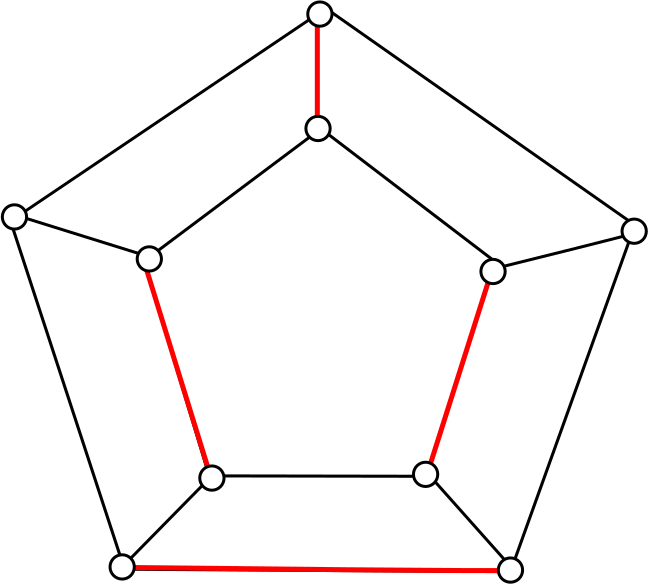
\includegraphics[width=5cm,height=4cm]{matching}
\end{frame}
\begin{frame}
  \frametitle{3. 匹配、霍尔定理}
  \begin{Def}
    设$Y$是图$G=(V,E)$的一个匹配,如果$2|Y|=|V|$,则称$Y$为$G$的一个\alert{完美匹配}。
  \end{Def}
\pause
\centering
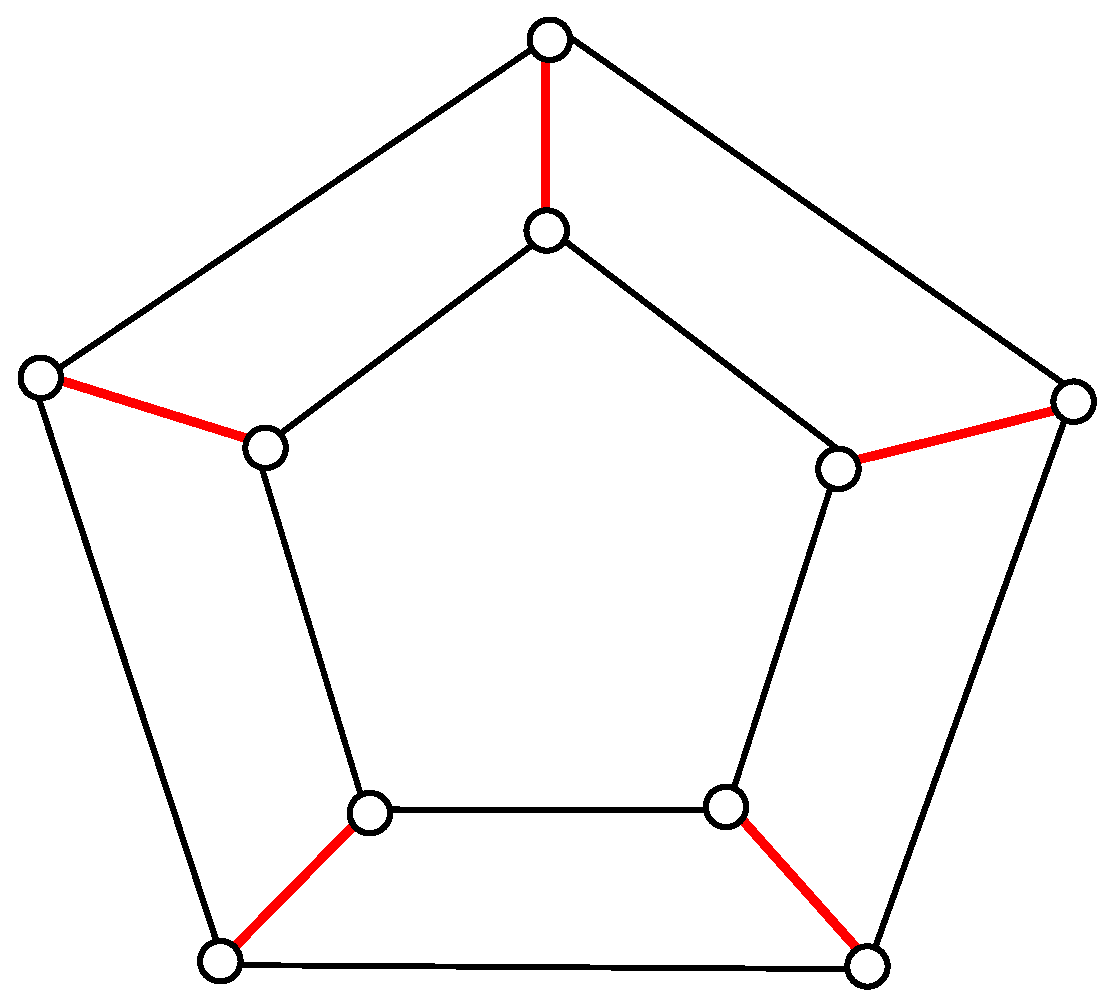
\includegraphics[width=5cm,height=4cm]{perfect}
\end{frame}

\begin{frame}
  \frametitle{3. 匹配、霍尔定理}

    \begin{Def}
   设$Y$是图$G=(V,E)$的一个匹配,如果对于$G$的任一匹配$Y'$,恒有$|Y'|\leq |Y|$, 则称$Y$为$G$的一个\alert{最大匹配}。
  \end{Def}
\pause
\centering
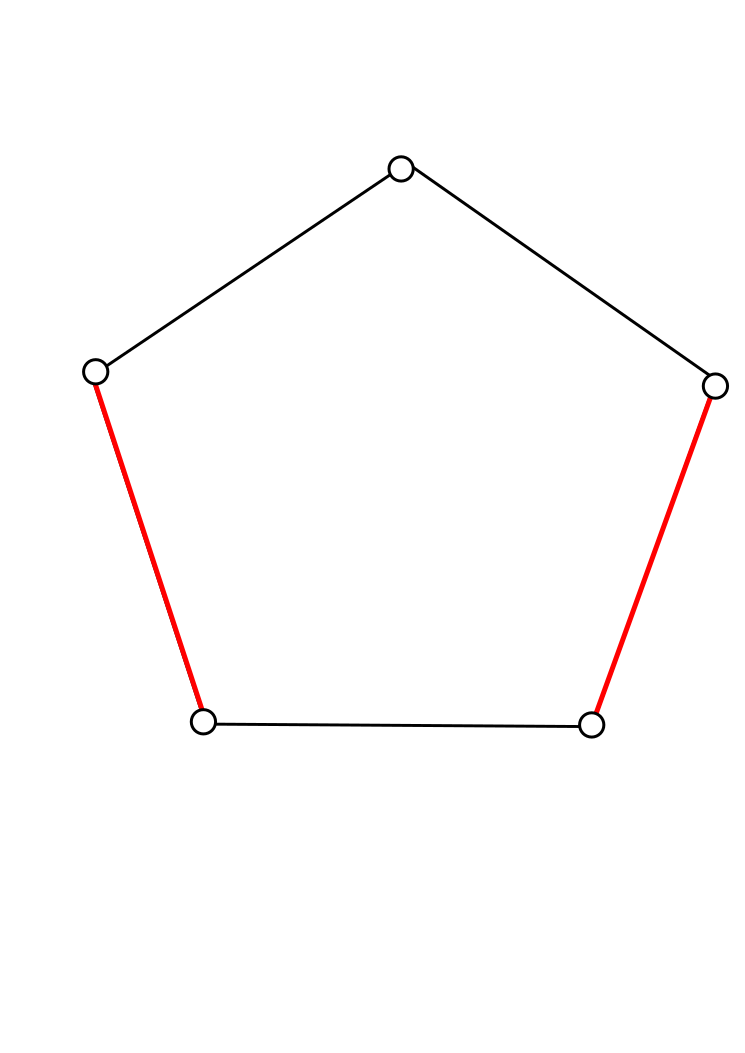
\includegraphics[width=4cm,height=3cm]{maximum}

\end{frame}
\begin{frame}
  \frametitle{3. 匹配、霍尔定理}

  \begin{Def}
    设$G=(V,E)$是一个偶图且$V=V_1\cup V_2$,
    $\forall x \in
    E$,$x$是联结$V_1$的一个顶点与$V_2$的一个顶点的边。如果存在$G$的一
    个匹配$Y$使得$|Y|=min\{|V_1|,|V_2|\}$,则称$Y$是偶图$G$的一个\alert{完全匹配}。
  \end{Def}

\end{frame}

\begin{frame}
  \frametitle{匹配}
  \begin{Thm}
    设$G=((V_1,V_2),E)$为偶图,存在$G$的一个完全匹配$Y$且$|Y| = |V_1|$的充分必要条件是对$V_1$的任意子集$A$, $|N(A)| \geq |A|$,其中\[N(A) = \{y\in V_2|\exists x \in A \{x,y\} \in E\}\]。
  \end{Thm}
\end{frame}

\end{CJK}
\end{document}

%%% Local Variables:
%%% mode: latex
%%% TeX-master: t
%%% End:
